\documentclass[11pt,letterpaper]{report}
\usepackage[latin1]{inputenc}
\usepackage{amsmath}
\usepackage{amsfonts}
\usepackage{amssymb}
\usepackage{graphicx}
\usepackage{color}
\usepackage{enumitem}
\usepackage[dvipsnames]{xcolor}
\definecolor{codegray}{gray}{0.9}
\newcommand{\code}[1]{\colorbox{codegray}{\texttt{#1}}}
\graphicspath{{../images/}{IR}}
%\newcommand{\LF}{}  % turn on to display large format
\ifdefined \LF
\usepackage[left=2.0cm, top=2.0cm, landscape]{geometry}  % for large format landscape
\else
\usepackage[left=2.0cm, top=2.0cm]{geometry}
\fi
\usepackage{fancyhdr}
\pagestyle{fancy}
\fancyhead{}
\lhead{CS350}
\chead{Dynamic Programming}
\rhead{Alexander DuPree}
\begin{document}

\ifdefined \LF
{\Large     % large print start
\fi

  \noindent\textbf{1. Modified Change Problem:}
  Apply the dynamic programming algorithm to find all the solutions to the change-making 
  problem for the denominations 1, 3, 5 and the amount $n = 9$.

  \begin{figure}[h!]
	\centering
	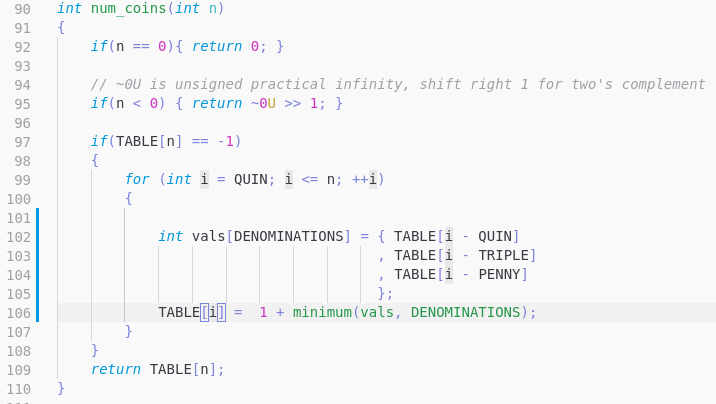
\includegraphics[width=1\linewidth]{num_coins.png}
	\caption[cs350]{Source code for Tabular make change algorithm}
	\label{fig:P1compileP0-1}
  \end{figure}

  \begin{figure}[h!]
	\centering
	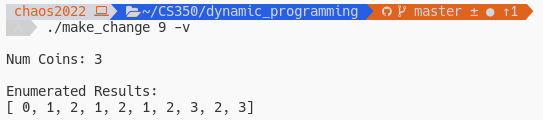
\includegraphics[width=1\linewidth]{num_coins_output.png}
	\caption[cs350]{Output for the make change program}
	\label{fig:P1compileP0-1}
  \end{figure}

  \pagebreak

  \noindent\textbf{2. Rod Cutting Problem}
  Design a dynamic programming algorithm for the following problem. Find the maximum 
  total sale price that can be obtained by cutting a rod of n units long in to 
  integer-length pieces if the sale price of a piece i units long is pi for i = 1, 2, 
  . . . , n.  What are the time and space efficiencies of your algorithm?

  \begin{figure}[h!]
	\centering
	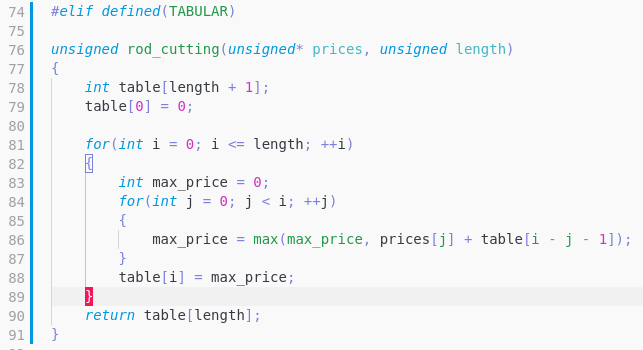
\includegraphics[width=1\linewidth]{rod_cutting.png}
	\caption[cs350]{Source code for tabular rod cutting algorithm}
	\label{fig:P1compileP0-1}
  \end{figure}

  This tabular algorithm has a space complexity of $\Theta(n)$ and a time 
  complexity of $\Theta(n^2)$, where n is the length of the rod. 

  \pagebreak

  \noindent\textbf{3. Minimum Sum Descent}: Find the smallest sum in 
  a descent from the triangle apex to its base through a sequence of adjacent 
  numbers. Design a dynamic programming algorithm for this problem and indicate 
  its time efficiency.

  \begin{figure}[h!]
	\centering
	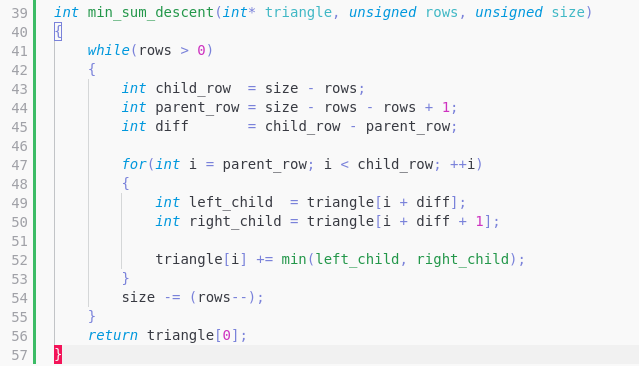
\includegraphics[width=1\linewidth]{sum_descent1.png}
	\caption[cs350]{Source code for tabular minimum sum descent algorithm}
	\label{fig:P1compileP0-1}
  \end{figure}

  This tabular algorithm has a space complexity of $\Theta(n^2)$, since to represent 
  the triangle we need to use at least $\sum_{i=1}^{n}i$ space. Likewise, the time 
  complexity is $\Theta(n^2)$ as well since for each element in each row up to $n-1$ 
  rows we must find the minimum value of the nodes children. I.E. $\sum_{i=1}^{n-1}i$ 
  work is done. 

  \pagebreak

  \noindent\textbf{4. N-Choose-K Problem}: Design a dynamic programming algorithm for the
  recursive n-choose-k problem discussed in class and then indicate its time and space 
  complexity.

  \begin{figure}[h!]
	\centering
	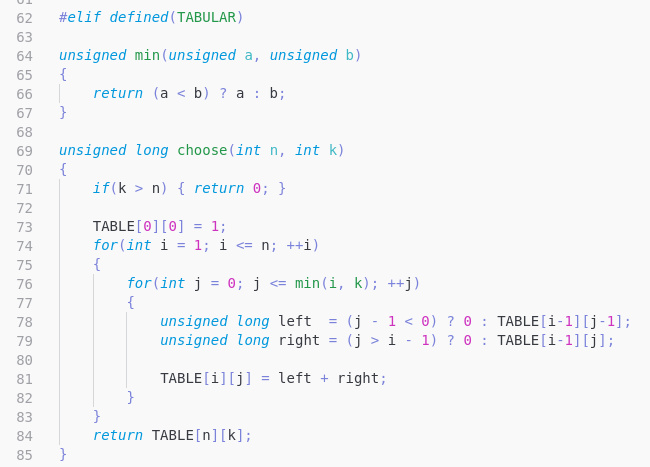
\includegraphics[width=1\linewidth]{choose1.png}
	\caption[cs350]{Source code for tabular binomial coefficient algorithm}
	\label{fig:P1compileP0-1}
  \end{figure}

  The time and space complexity for this tabular algorithm are both $\Theta(n\cdot k)$

  \pagebreak

  \noindent\textbf{5. Pebble Collecting Problem}: Design a dynamic problem solution 
  for the pebble collecting problem described in class, and indicate its time 
  and space efficiency. 

  \begin{figure}[h!]
	\centering
	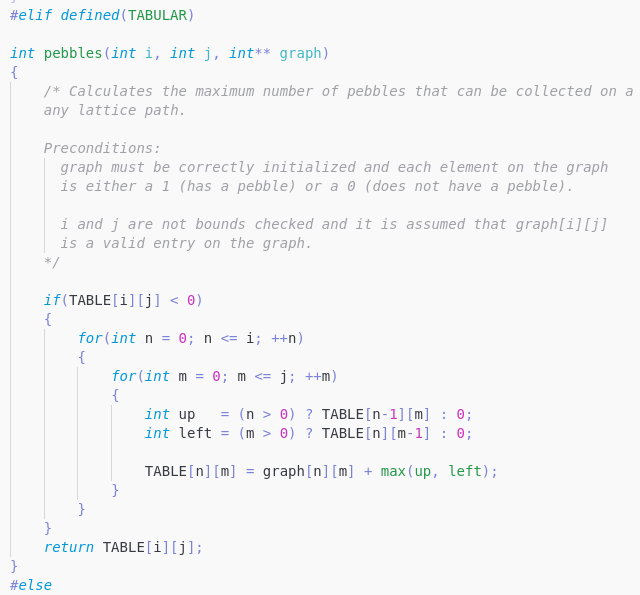
\includegraphics[width=1\linewidth]{pebbles1.png}
	\caption[cs350]{Source code for tabular pebble collecting algorithm}
	\label{fig:P1compileP0-1}
  \end{figure}

  The time and space complexity for this tabular algorithm are both $\Theta(n \cdot m)$
  where $n$ and $m$ are the dimensions of the graph. 

\ifdefined \LF
} % large print end
\fi

\end{document}